\section{ASK-Modulation vom Leseger\"at zum Tag}
In dieser Aufgabe wird die Signal\"ubertragung vom Leseger\"at zum RFID-Tag untersucht. Ziel ist es, die Amplitudenumtastung (ASK) des Tr\"agersignals sichtbar zu machen und zu zeigen, dass das modulierte HF-Signal am Tag wieder als niederfrequentes Nutzsignal gewonnen werden kann.

\subsection{Schaltung}
Die Gesamtschaltung besteht aus der Sendestufe des Leseger\"ats in \cref{fig:lesegeraet_ask_schaltung} und der Empfangsstufe des Tags in \cref{fig:tag_ask_schaltung}. Das Leseger\"at erzeugt das magnetische Wechselfeld und schaltet dessen Amplitude mit einem Rechtecksignal periodisch ein und aus. Dadurch entsteht ein amplitudenmoduliertes Tr\"agersignal.

Am Tag wird dieses Signal \"uber den Resonanzkreis aufgenommen. Hinter der Gleichrichtung beziehungsweise H\"ullkurvenbildung kann das niederfrequente Modulationssignal wieder beobachtet werden. Damit wird gezeigt, dass Informationen nicht nur vom Tag zum Leseger\"at, sondern auch in Gegenrichtung \"ubertragen werden k\"onnen.

\begin{figure}[H]
  \centering
  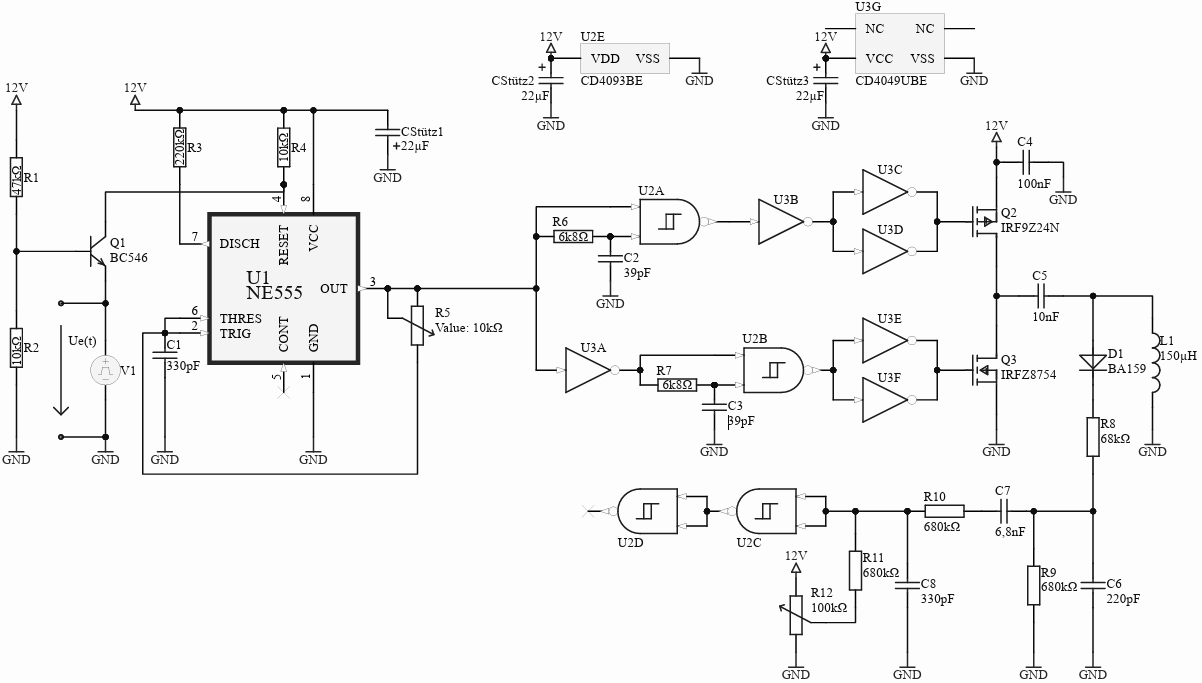
\includegraphics[width=0.9\linewidth]{Schaltungen/Lesegeraet_ModulationVonTag}
  \caption{Schaltung des Leseger\"ats zur ASK-Modulation}
  \label{fig:lesegeraet_ask_schaltung}
\end{figure}

\begin{figure}[H]
  \centering
  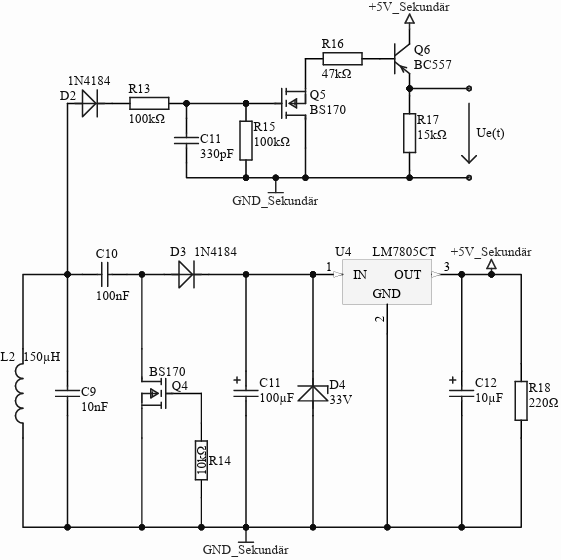
\includegraphics[width=0.5\linewidth]{Schaltungen/Tag_ModulationVonTag}
  \caption{Schaltung des Tags zum Empfang der ASK-Modulation}
  \label{fig:tag_ask_schaltung}
\end{figure}

\subsection{Messvorgang}
Als Träger der Modulation wird das Ausgangssignal des NE555 verwendet, welches periodisch über einen Funktionsgenerator geschalten wird (ON-OFF-Keying). Dieses Rechtecksignal schaltet die Sendestufe des Leseger\"ats periodisch ein und aus. F\"ur die Messung werden nacheinander das Steuersignal des NE555, das modulierte Signal auf der Prim\"arseite des Leseger\"ats, das eingekoppelte Signal am Tag sowie das demodulierte Ausgangssignal des Tags mit dem Oszilloskop aufgenommen.

Dabei wird untersucht, ob das vom Leseger\"at vorgegebene Rechtecksignal entlang der gesamten \"Ubertragungskette wiedererkennbar bleibt. Insbesondere soll gezeigt werden, dass sich die Ein- und Ausschaltvorg\"ange des HF-Tr\"agers am Tag nach der Demodulation erneut als niederfrequenter Rechteckverlauf darstellen lassen.

\subsection{Messergebnis}
In \cref{fig:ask_ne555_out} ist auf CH1 das Steuerungssignal der Modulation zu erkennen. Auf CH2 ist das Signal am Ausgang des NE555 zu sehen. Wie zu erwarten wird je nach Status des Funktionsgenerators das Rechtecksignal des NE555 aktiviert oder deaktiviert und erzeugt dann eine H\"ullkurve von $495\,Hz$.

Die Wirkung auf das HF-Signal des Leseger\"ats ist in \cref{fig:ask_primaer_out} erkennbar. Auf CH1 ist der Eingang beziehungsweise das Reset-/Run-Signal zu sehen, auf CH2 das daraus entstehende ASK-Signal auf der Prim\"arseite. Die Tr\"agerschwingung ist nur w\"ahrend der High-Phasen des Steuersignals vorhanden. Dadurch entsteht die Amplitudenumtastung des Sendesignals.

In \cref{fig:ask_sekundaer_in} ist das auf den Tag \"ubertragene Signal dargestellt. Auch hier zeigt CH1 den Eingang beziehungsweise das Reset-/Run-Signal und CH2 das ASK-Signal am Tag. Das modulierte Tr\"agersignal wird \"uber die induktive Kopplung auf den Resonanzkreis des Tags \"ubertragen und liegt dort mit kleinerer Amplitude, aber gleichem zeitlichem Verlauf vor.

Besonders deutlich wird das Ergebnis in \cref{fig:ask_sekundaer_out}. CH1 zeigt den Eingang beziehungsweise das Reset-/Run-Signal, CH2 zeigt das ASK-Signal nach der Empfangs- beziehungsweise Demodulationsstufe. Nach der Gleichrichtung und Gl\"attung am Tag wird aus dem amplitudenmodulierten HF-Signal wieder ein niederfrequenter Spannungsverlauf. Dieser folgt dem urspr\"unglichen Rechtecksignal des Leseger\"ats und best\"atigt damit die erfolgreiche ASK-\"Ubertragung vom Leseger\"at zum Tag.

\begin{figure}[H]
  \centering
  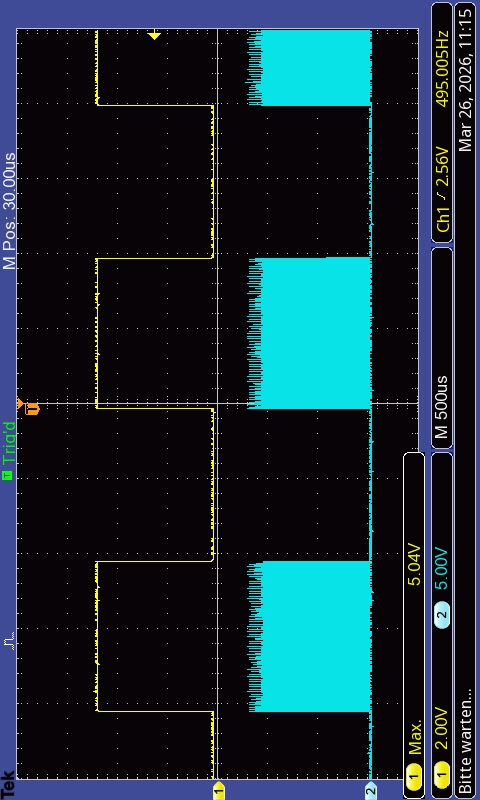
\includegraphics[width=0.42\linewidth, angle=-90]{Modulation_Lesegeraet--Tag/NE555_Out}
  \caption{Steuersignal des NE555 f\"ur die ASK-Modulation}
  \label{fig:ask_ne555_out}
\end{figure}

\begin{figure}[H]
  \centering
  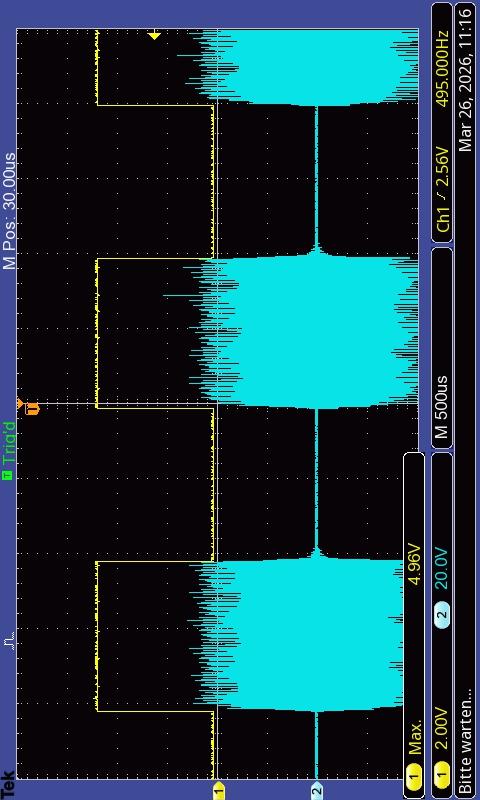
\includegraphics[width=0.42\linewidth, angle=-90]{Modulation_Lesegeraet--Tag/Primaer_Out}
  \caption{ASK-moduliertes Signal auf der Prim\"arseite des Leseger\"ats}
  \label{fig:ask_primaer_out}
\end{figure}

\begin{figure}[H]
  \centering
  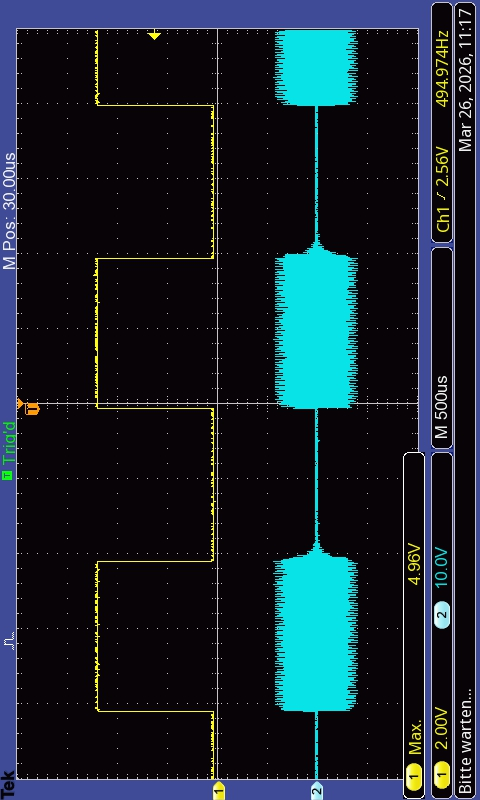
\includegraphics[width=0.42\linewidth, angle=-90]{Modulation_Lesegeraet--Tag/Sekundaer_In}
  \caption{Am Tag eingekoppeltes ASK-Signal}
  \label{fig:ask_sekundaer_in}
\end{figure}

\begin{figure}[H]
  \centering
  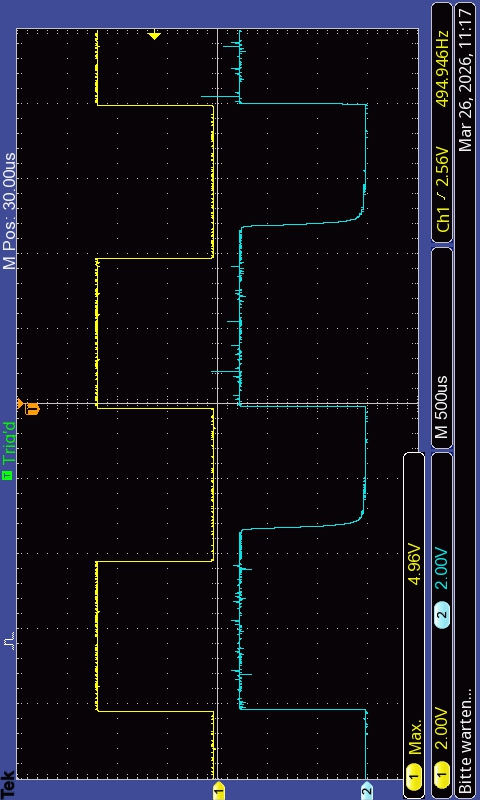
\includegraphics[width=0.42\linewidth, angle=-90]{Modulation_Lesegeraet--Tag/Sekundaer_out}
  \caption{Demoduliertes Ausgangssignal am Tag}
  \label{fig:ask_sekundaer_out}
\end{figure}

\subsection{Interpretation}
Die Messung zeigt, dass das Leseger\"at Informationen \"uber ASK erfolgreich zum Tag \"ubertragen kann. Das Rechtecksignal des NE555 ist der HF-Tr\"ager, wodurch auf der Prim\"arseite ein getastetes Sendesignal entsteht. Dieses wird \"uber die magnetische Kopplung auf den Tag \"ubertragen.

Am Tag kann das Signal nach der H\"ullkurvenbildung wieder als niederfrequenter Verlauf erkannt werden. Damit ist nachgewiesen, dass die Informations\"ubertragung vom Leseger\"at zum Tag funktioniert und sich das Modulationssignal am Empf\"anger wiedergewinnen l\"asst.
